\documentclass[twocolumn, a4j,10pt]{jarticle}

%%% use package
\usepackage[utf8]{inputenc}
\usepackage{bm}
\usepackage{array}
\usepackage{dcolumn}
\usepackage{caption}
\usepackage{subcaption}
\usepackage{sty/cite}
\usepackage{here}
\usepackage{amssymb,amsmath,nidanfloat}
\usepackage[dvipdfmx]{graphicx}
\usepackage[dvipdfmx]{color}
\usepackage{fancybox,ascmac}
\usepackage{color}
\usepackage{url}
\usepackage{latexsym}
\usepackage{csquotes}
\usepackage{nomencl}
\usepackage{multirow}

\usepackage{algorithm}
\usepackage{algorithmic}
\usepackage[vdivide={5mm,,20mm},hdivide={10mm,30mm,10mm}]{geometry}
\usepackage{multicol}

%\setlength{\textwidth}{48zw}
%\setlength{\columnsep}{2zw}



\title{ロボットに対する道徳的態度に文化的背景が与える影響:\\宗教に着目した日米大規模比較調査による実証}
\author{五十里 翔吾}
\date{令和4年2月1日}
\DeclareRelationFont{JY1}{mc}{it}{}{OT1}{cmr}{it}{}
\DeclareRelationFont{JT1}{mc}{it}{}{OT1}{cmr}{it}{}
\DeclareFontShape{JY1}{mc}{m}{it}{<5> <6> <7> <8> <9> <10> sgen*min
    <10.95><12><14.4><17.28><20.74><24.88> min10
    <-> min10}{}
\DeclareFontShape{JT1}{mc}{m}{it}{<5> <6> <7> <8> <9> <10> sgen*tmin
    <10.95><12><14.4><17.28><20.74><24.88> tmin10
    <-> tmin10}{}
\DeclareRelationFont{JY1}{mc}{sl}{}{OT1}{cmr}{sl}{}
\DeclareRelationFont{JT1}{mc}{sl}{}{OT1}{cmr}{sl}{}
\DeclareFontShape{JY1}{mc}{m}{sl}{<5> <6> <7> <8> <9> <10> sgen*min
    <10.95><12><14.4><17.28><20.74><24.88> min10
    <-> min10}{}
\DeclareFontShape{JT1}{mc}{m}{sl}{<5> <6> <7> <8> <9> <10> sgen*tmin
    <10.95><12><14.4><17.28><20.74><24.88> tmin10
    <-> tmin10}{}
\DeclareRelationFont{JY1}{mc}{sc}{}{OT1}{cmr}{sc}{}
\DeclareRelationFont{JT1}{mc}{sc}{}{OT1}{cmr}{sc}{}
\DeclareFontShape{JY1}{mc}{m}{sc}{<5> <6> <7> <8> <9> <10> sgen*min
    <10.95><12><14.4><17.28><20.74><24.88> min10
    <-> min10}{}
\DeclareFontShape{JT1}{mc}{m}{sc}{<5> <6> <7> <8> <9> <10> sgen*tmin
    <10.95><12><14.4><17.28><20.74><24.88> tmin10
    <-> tmin10}{}
\DeclareRelationFont{JY1}{gt}{it}{}{OT1}{cmbx}{it}{}
\DeclareRelationFont{JT1}{gt}{it}{}{OT1}{cmbx}{it}{}
\DeclareFontShape{JY1}{mc}{bx}{it}{<5> <6> <7> <8> <9> <10> sgen*goth
    <10.95><12><14.4><17.28><20.74><24.88> goth10
    <-> goth10}{}
\DeclareFontShape{JT1}{mc}{bx}{it}{<5> <6> <7> <8> <9> <10> sgen*tgoth
    <10.95><12><14.4><17.28><20.74><24.88> tgoth10
    <-> tgoth10}{}
\DeclareRelationFont{JY1}{gt}{sl}{}{OT1}{cmbx}{sl}{}
\DeclareRelationFont{JT1}{gt}{sl}{}{OT1}{cmbx}{sl}{}
\DeclareFontShape{JY1}{mc}{bx}{sl}{<5> <6> <7> <8> <9> <10> sgen*goth
    <10.95><12><14.4><17.28><20.74><24.88> goth10
    <-> goth10}{}
\DeclareFontShape{JT1}{mc}{bx}{sl}{<5> <6> <7> <8> <9> <10> sgen*tgoth
    <10.95><12><14.4><17.28><20.74><24.88> tgoth10
    <-> tgoth10}{}
\DeclareRelationFont{JY1}{gt}{sc}{}{OT1}{cmbx}{sc}{}
\DeclareRelationFont{JT1}{gt}{sc}{}{OT1}{cmbx}{sc}{}
\DeclareFontShape{JY1}{mc}{bx}{sc}{<5> <6> <7> <8> <9> <10> sgen*goth
    <10.95><12><14.4><17.28><20.74><24.88> goth10
    <-> goth10}{}
\DeclareFontShape{JT1}{mc}{bx}{sc}{<5> <6> <7> <8> <9> <10> sgen*tgoth
    <10.95><12><14.4><17.28><20.74><24.88> tgoth10
    <-> tgoth10}{}
\DeclareRelationFont{JY1}{gt}{it}{}{OT1}{cmr}{it}{}
\DeclareRelationFont{JT1}{gt}{it}{}{OT1}{cmr}{it}{}
\DeclareFontShape{JY1}{gt}{m}{it}{<5> <6> <7> <8> <9> <10> sgen*goth
    <10.95><12><14.4><17.28><20.74><24.88> goth10
    <-> goth10}{}
\DeclareFontShape{JT1}{gt}{m}{it}{<5> <6> <7> <8> <9> <10> sgen*tgoth
    <10.95><12><14.4><17.28><20.74><24.88> tgoth10
    <-> tgoth10}{}
\endinput


\begin{document}

\maketitle
\vspace{-7mm}
\subsection*{概要}\vspace{-3mm}
ロボットに対して、人は道徳心をもつのだろうか。ロボットに対する攻撃を受け入れがたいと感じる人が数多く存在することを示す実例はいくつか存在する。例えば、ロボットが蹴られている動画に対して否定的なコメントがなされる、街で破壊されたロボットを見た人が、それを壊した人を非難する投稿を行うなどといった事例である。


キリスト教のような啓示宗教の伝統では、人間は他の存在とは異なる最も重要な存在であるという人間中心主義が影響力を持っている。一方で、神道や仏教の伝統では、人とそれ以外の間に明確な区別が無く、どちらも同じ法則に従うというアニミズム的価値観が影響力を持っている。このような宗教的伝統の違いは「人間ではない存在」であるロボットに対する態度に影響を与えると考えられている。しかし、ロボットに対する道徳に着目して宗教的伝統の影響を実証した研究は存在しない。本研究では、キリスト教の伝統を持つアメリカと、神道・仏教の伝統を持つ日本を対象に、宗教的伝統がロボットに対する道徳的配慮に与える影響を比較した。
\vspace{-7mm}
\subsection*{仮説と方法} \vspace{-3mm}
本研究で検討した仮説は以下である。1)日本のほうがアメリカよりもロボットに対する道徳的配慮が強い。2)アメリカ(人間中心主義的伝統の影響下)では、宗教心の強さはロボットに対する道徳的配慮に負の影響を与え、日本(アニミズム的伝統の影響下)では、正の影響を与える。これら仮説を検証するため、大規模な質問紙調査を実施した(N=3,781)。
測定した変数は、ロボットに対する道徳的配慮、宗教心の強さ、人間中心主義傾向、アニミズム傾向である。共変量として、性別、年齢、教育歴、他人に対する感受性の強さ、ロボットに触れた経験という要因を統制した。
\vspace{-7mm}
\subsection*{明らかにしたこと}\vspace{-3mm}
仮説1)で予想したとおり、日本の被験者のほうがロボットに対する道徳的配慮が高いという結果が得られた。この結果は、西洋に比べて日本がロボットに受容的、親和的であるという既存の研究結果[1]と符合するものである。仮説2)に関する結果は、一部が仮説通りであった。まず、アメリカでのみ宗教心の強さがロボットに対する道徳的配慮に弱い負の影響を持っていた。一方で、日本では正負どちらの影響も見られなかった。
宗教心、人間中心主義傾向、アニミズム傾向を考慮したパスモデルによる解析では、両国において同様の構造が見いだされた(図1)。具体的には、宗教心は人間中心主義、アニミズム双方に正の影響を持っていた。また、人間中心主義は負の影響を、アニミズムは正の影響をロボットに対する道徳的配慮に与えていた。
ただし、アメリカにおいては宗教心が人間中心主義に与える影響がより強く、日本においては宗教心がアニミズムに与える影響がより強いといった文化差の存在も見いだされた。
\begin{figure}[H]
 \centering
 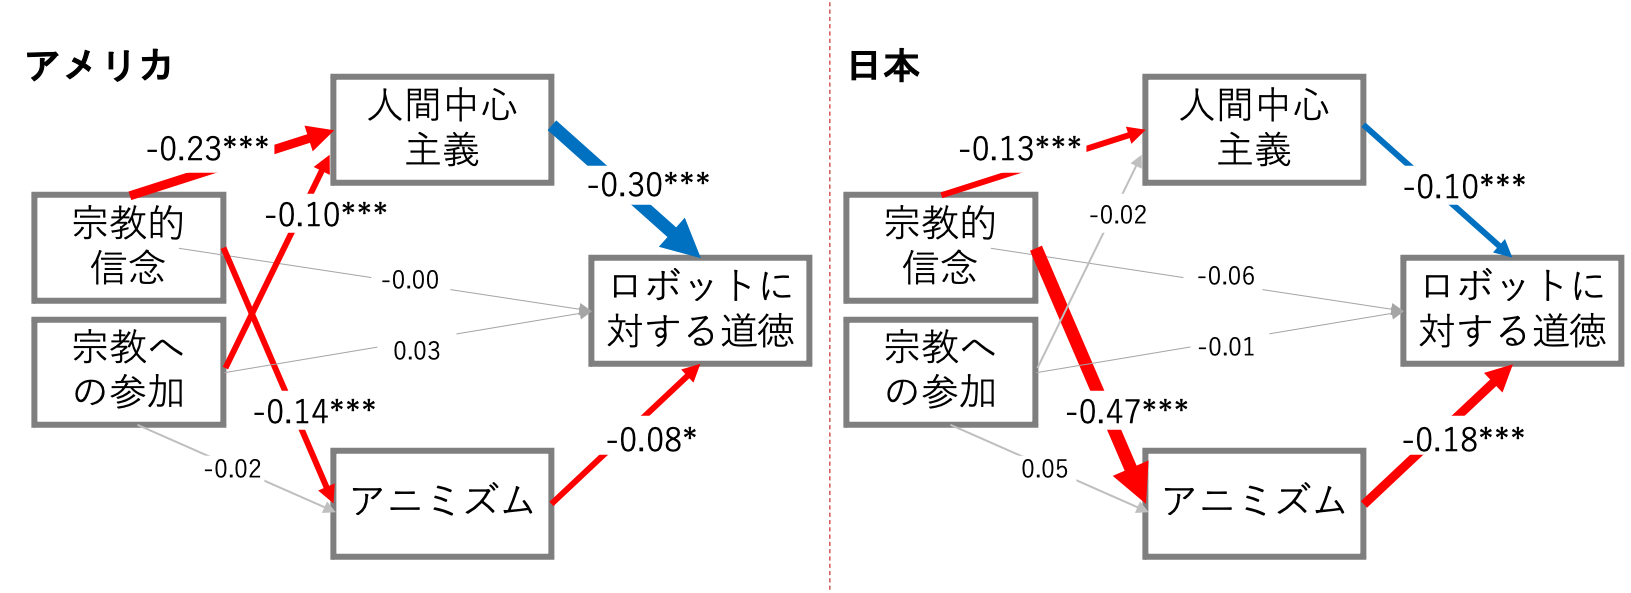
\includegraphics[keepaspectratio, width=9.5cm]{images/sem2.png}
 \caption{Mult-group SEMによるパス解析の結果}
 \label{sem}
\end{figure}

\vspace{-7mm}
\subsection*{本研究の意義}\vspace{-3mm}
これまでの研究では、ロボットに対する受容性や親和性における文化差が検討されてきたが、本研究はロボットに対する道徳を扱うことで新たな研究領域を開拓した。ロボット対する人の道徳心を定量化することで、昨今の技術倫理で議論されている「ロボットに対して人はどう振る舞うのが望ましいのか」という主題に対する実証的データを提供する。大規模かつ偏りのないサンプルを用いたことで、結果の妥当性も高い。また、宗教によって動機づけられた価値観がロボットに対する道徳的配慮にどのような影響を与えるかに着目するアプローチは先例がなく新規性が高い。このような研究方法をとったことから、文化差のあるなしだけではなく、それらを生じさせる文化的要因に踏み込んだ理論的な検討が可能となった。さらに、本研究の発見は、異なる文化においては異なるインタラクションデザインをロボットに実装する必要があるという可能性[2]を実証的に示す。\vspace{-4mm}
\thispagestyle{empty}
\subsection*{参考文献}\vspace{-3mm}{\footnotesize
[1] MacDorman, K. F., Vasudevan, S. K., \& Ho, C. C. (2009). Does Japan really have robot mania? Comparing attitudes by implicit and explicit measures. \textsl{AI \& society, 23}(4), 485-510.\\ \relax
[2] \v{S}abanovi\'{c}, S., Bennett, C. C., \& Lee, H. R. (2014, March). Towards culturally robust robots: A critical social perspective on robotics and culture. In \textsl{Proc. HRI Workshop on Culture-Aware Robotics (Vol. 2014)}.}
\end{document}






